
\section{Part III - Luenberger observer}



The Luenberger observer is introduced to improve the state estimation process in the helicopter lab. In previous labs, we relied solely on the Inertial Measurement Unit(IMU) for measurements like angular rates and accelerations. While useful, the IMU suffers from sensor noise, errors in angular estimation, and sensitivity to its position near the lever arm, which affects data accuracy.
\vspace{1em}

Positioning of the IMU influences the data. And the IMU is centered more in the middle of the lever arm, which influences the data.
By use of the Luenberger observer mathematical model we can improve the measurements.
\vspace{1em}

\section{Lab Preparation}
\title{\textbf{Extended state-space formulation}}
\maketitle
\vspace{1em}


Given the basis of
\[
x =
\begin{bmatrix}
{p} \\
\dot{p}\\
{e} \\
\dot{e} \\

\dot{{\lambda}} \\


\end{bmatrix}, \quad
u =
\begin{bmatrix}
\tilde{V}_s \\
V_d
\end{bmatrix}, \quad
\]

Based on the variables we get the following state-space model matrixes:

\[
A = \begin{bmatrix}
0 & 1 & 0 & 0 & 0 \\
0 & 0 & 0 & 0 & 0 \\
0 & 0 & 0 & 1 & 0 \\
0 & 0 & 0 & 0 & 0 \\
K_3 & 0 & 0 & 0 & 0 \\
\end{bmatrix}, \quad
B = \begin{bmatrix}
0 & 0 \\
0 & K_1 \\
0 & 0 \\
K_2 & 0 \\
0 & 0 \\
\end{bmatrix}, \quad
C = \begin{bmatrix}
0 & 0 & 1 & 0 & 0 \\
0 & 0 & 0 & 0 & 1 \\

\end{bmatrix}.
\]

\vspace{2em}
\noindent
\noindent
\title{\textbf{Observability}}

\maketitle
\vspace{2em}

The observability matrix is the following:
\[
O =
\begin{bmatrix}
C \\
CA \\
\vdots \\
CA^{n-1}
\end{bmatrix}
\]


\noindent
The system is Observable. Which makes it possible to infer states of the system. So you can effectively monitor or control the system.
The minimum set of states you need is e, and lambda that still makes the system observable. 


\vspace{1em}


\noindent
\title{ \textbf{State estimator}} 
\maketitle
\vspace{1em}
\vspace{1em}

\[
\dot{\hat{x}} = \hat{A}x + Bu + L(y - \hat{C}x)
\]

\vspace{1em}



\noindent
We just used the 
L=place(A',C',P) command in matlab. P is a vector of the wanted poles.
Like the following example:

\[
P = \begin{bmatrix}
-9 \\
-9 \\
-9 \\
-9 \\
-9
\end{bmatrix}
\]

\vspace{1em}



\noindent
 Since the system is observable, it is possible to place the poles of the estimator arbitrarily
 by choosing an appropriate gain matrix, L. The poles of the estimator is the same as
 the poles of A-LC. 
 

 \vspace{1em}
\noindent
 \title{{\textbf{Test plan}}
 \maketitle
 \vspace{1em}


Trying different values of poles. 
From small absolute values to bigger in the Left Half Plane.
We tried pole values: -2, -9 ,-90.
The reasoning was that smaller values of poles will correspond to slower estimation and a slower convergence rate which has more lag. On the other hand model uncertainties will be increased with too big values of poles. The helicopter lab has states that change quickly. So we thought bigger pole values would be better.
The first value was bad, the second was okay, and the third had a good smooth result but had a offset.
\vspace{2em}
For the smaller pole values the estimates are less accurate. And for the larger pole values there is a offset(lag). 
For some estimates the difference is hard to spot like for the measurement and estimator for the apple figures.
The difference between small and big pole values can clearly be seen between Blueberry 1(figure z) and Blueberry 4(figure y). 
For the smaller pole values the estimates are less accurate. And for the larger pole values there is a offset(lag). 
For some estimates the difference is hard to spot like for the Apples.
The difference between small and big pole values can clearly be seen between Blueberry 1(figure z) and Blueberry 4(figure y). 
Blueberry 1 is a faster estimator with more noise. Which corresponds to bigger absolute values of the poles.
Blueberry 4 is a slower estimator with more lag which corresponds to lower absolute pole values. 


\title{\textbf{Conclusion}}
\maketitle
\vspace{2em}






\noindent
The pitch estimations appears to be more inaccurate the faster you try to
to sample a state, and limitations to the observer has to be implemented to
make the system stable.
The L matrix in the observer scales the deviation between the measured and
estimated states.
\noindent
Based on the plots, the elevation estimation seems to be working correctly as
it has very few deviations from the actual measurement.


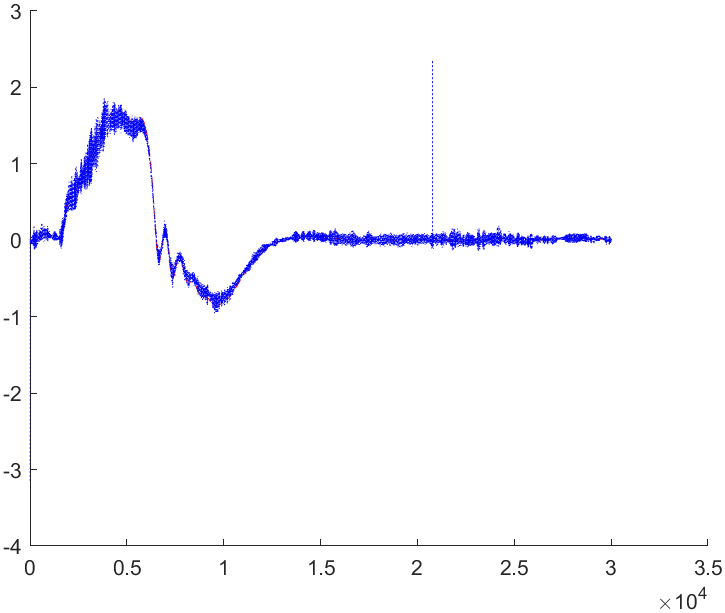
\includegraphics{LabTest1(Apple)fixed.png}
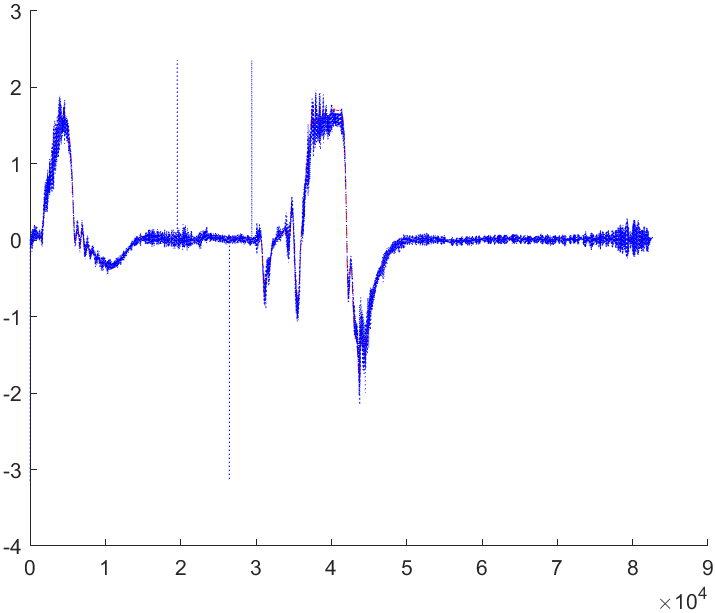
\includegraphics{LabTest2(Apple)fixed.png}

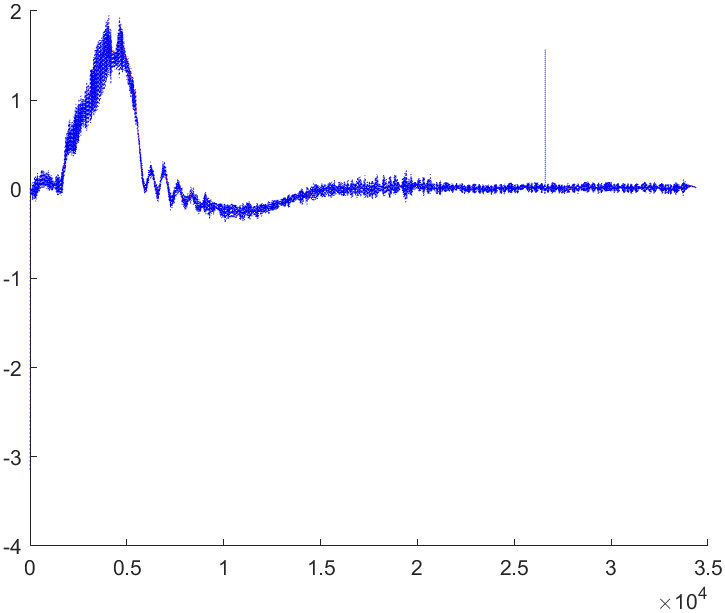
\includegraphics{LabTest3(Apple)fixed.png}
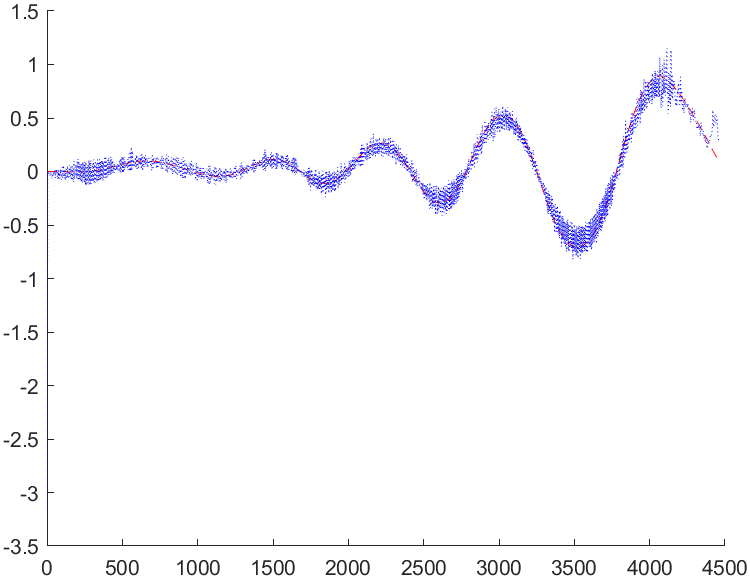
\includegraphics{LabTest4(Apple)fixed.png}


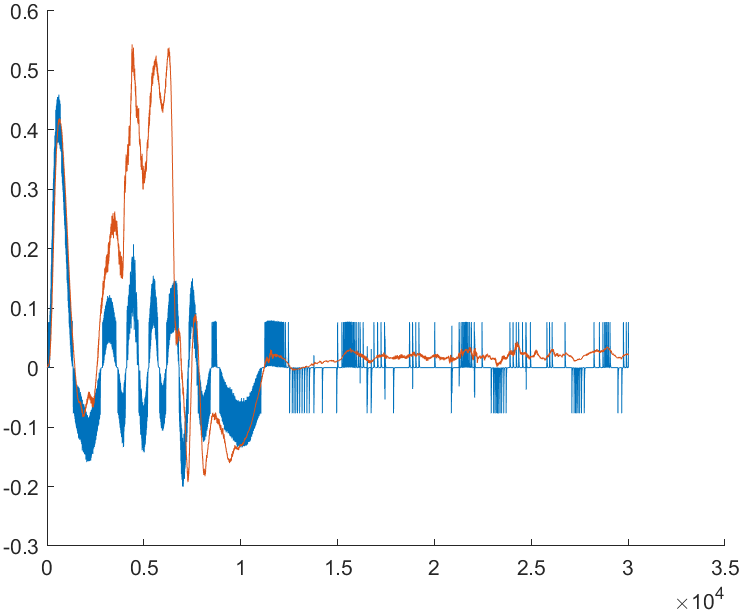
\includegraphics{LabTest1(Blueberry).png}
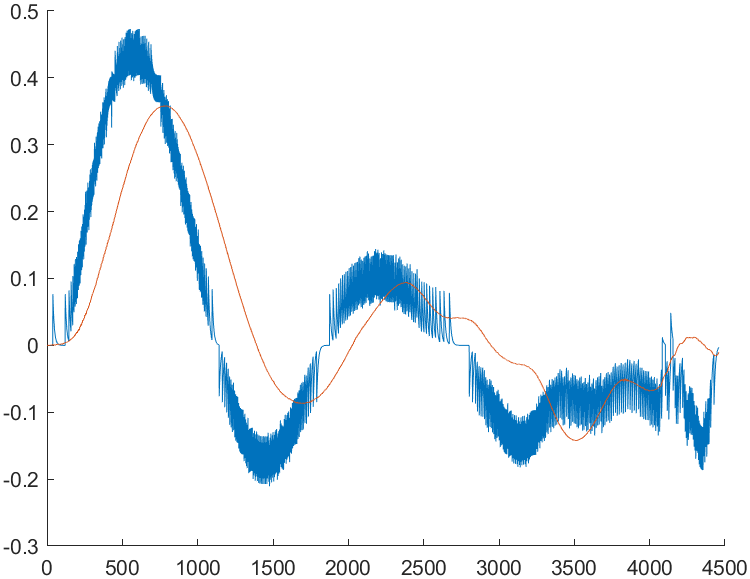
\includegraphics{LabTest4(Blueberry).png}

